% yaml_workflow_v2.tex
% Alternative workflow diagram - Simpler horizontal flow
% Author: João Pedro Azevedo
% Date: December 2025

\documentclass[tikz,border=10pt]{standalone}
\usepackage{tikz}
\usetikzlibrary{shapes.geometric, arrows.meta, positioning, fit, backgrounds, calc}

\begin{document}

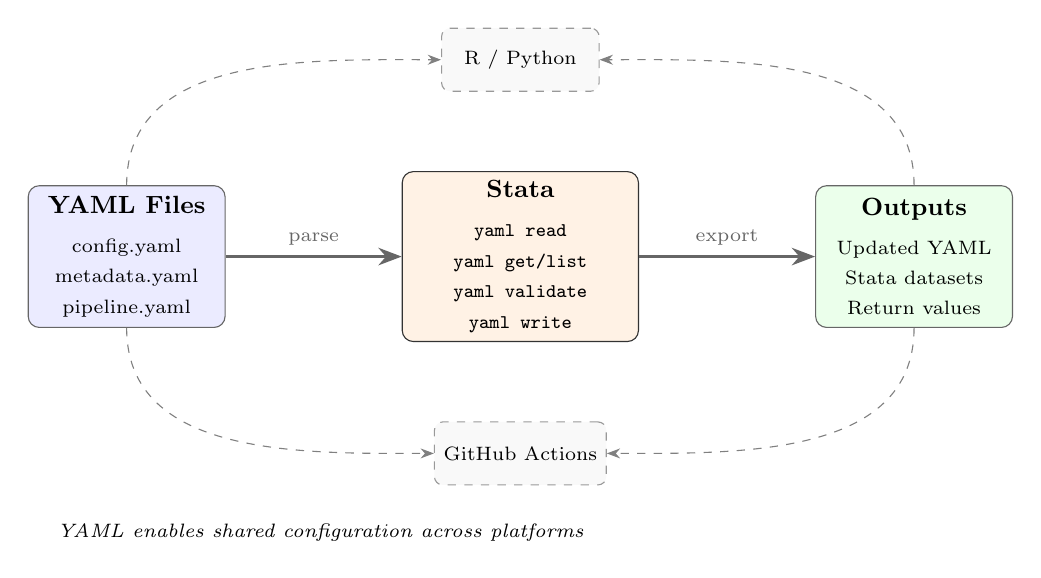
\begin{tikzpicture}[
    % Node styles
    configbox/.style={
        rectangle, 
        rounded corners=4pt,
        draw=black!60, 
        fill=blue!8,
        minimum width=2.5cm, 
        minimum height=1.8cm,
        font=\small,
        align=center
    },
    statabox/.style={
        rectangle, 
        rounded corners=4pt,
        draw=black!80, 
        fill=orange!10,
        minimum width=3cm, 
        minimum height=2cm,
        font=\small,
        align=center
    },
    outputbox/.style={
        rectangle, 
        rounded corners=4pt,
        draw=black!60, 
        fill=green!8,
        minimum width=2.5cm, 
        minimum height=1.8cm,
        font=\small,
        align=center
    },
    arrow/.style={
        ->,
        >=Stealth,
        very thick,
        black!60
    }
]

% === Input (Left) ===
\node[configbox] (input) at (0, 0) {
    \textbf{YAML Files}\\[3pt]
    {\scriptsize config.yaml}\\
    {\scriptsize metadata.yaml}\\
    {\scriptsize pipeline.yaml}
};

% === Stata Processing (Center) ===
\node[statabox] (stata) at (5, 0) {
    \textbf{Stata}\\[3pt]
    {\ttfamily\scriptsize yaml read}\\
    {\ttfamily\scriptsize yaml get/list}\\
    {\ttfamily\scriptsize yaml validate}\\
    {\ttfamily\scriptsize yaml write}
};

% === Output (Right) ===
\node[outputbox] (output) at (10, 0) {
    \textbf{Outputs}\\[3pt]
    {\scriptsize Updated YAML}\\
    {\scriptsize Stata datasets}\\
    {\scriptsize Return values}
};

% === Arrows ===
\draw[arrow] (input) -- node[above, font=\scriptsize] {parse} (stata);
\draw[arrow] (stata) -- node[above, font=\scriptsize] {export} (output);

% === Cross-platform sharing ===
\node[rectangle, draw=black!40, dashed, rounded corners=3pt, fill=gray!5,
      minimum width=2cm, minimum height=0.8cm, font=\scriptsize, align=center] 
      (r) at (5, 2.5) {R / Python};
\node[rectangle, draw=black!40, dashed, rounded corners=3pt, fill=gray!5,
      minimum width=2cm, minimum height=0.8cm, font=\scriptsize, align=center] 
      (gh) at (5, -2.5) {GitHub Actions};

\draw[->, >=Stealth, dashed, black!50] (input) to[out=90, in=180] (r);
\draw[->, >=Stealth, dashed, black!50] (output) to[out=90, in=0] (r);
\draw[->, >=Stealth, dashed, black!50] (input) to[out=-90, in=180] (gh);
\draw[->, >=Stealth, dashed, black!50] (output) to[out=-90, in=0] (gh);

% === Legend ===
\node[font=\scriptsize, anchor=west] at (-1, -3.5) {\textit{YAML enables shared configuration across platforms}};

\end{tikzpicture}

\end{document}
